\documentclass[12pt,oneside,a4paper,landscape]{article}
\usepackage{pgf,tikz}
\usetikzlibrary{patterns,arrows}
%Configure page layout: a4, margin 0.79in, onesided, indent 0.5in
\paperwidth=8.27in
\paperheight=11.69in
\voffset=-0.21in
\hoffset=-0.21in
\oddsidemargin=0in
\evensidemargin=0in
\topmargin=-23pt
\headheight=12pt
\headsep=25pt
\marginparsep=0in
\marginparwidth=0in
\footskip=30pt
\marginparpush=0in
\textwidth=6.69in
\textheight=9.61in
%indent of a first line of new paragraphc is 0.5in to use \indent or \par
\parindent=0.5in
%set distance btw lines
\baselineskip=0pt
%set disctance btw pars
\parskip=0pt
\begin{document}
	\begin{list}{$\clubsuit$}{\parskip=0in \topsep=0in \itemsep=0in \parsep=0in \partopsep=0in 			\leftmargin=0in \rightmargin=0in \itemindent=0in \listparindent=\itemindent}
		\tikzstyle{circleNode}=[circle,draw=black,thick,inner sep=0pt,minimum size=7mm]
		\tikzstyle{rectangleNode}=[rectangle,draw=black,thick,inner sep=0pt,minimum width=12mm,minimum height=7mm]
		\tikzstyle{invisibleCircleNode}=[circle,inner sep=0pt,minimum size=4mm]
		\item Hinh 1
		%Raw command
			\begin{center}
				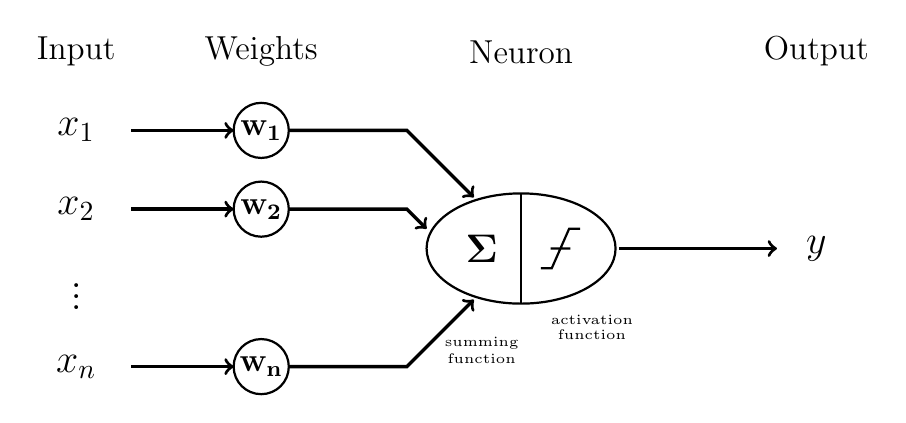
\begin{tikzpicture}
					\node at (0,0) {\large Input};
					\node at (0,-1cm) {\Large $x_1$};
					\node at (0,-2cm) {\Large $x_2$};
					\node at (0,-3cm) {\Large $\vdots$};
					\node at (0,-4cm) {\Large $x_n$};	
					\pgftransformxshift{0.7cm}	
					\draw[very thick,->] (0,-1cm) --++(1.3cm,0);	
					\draw[very thick,->] (0,-2cm) --++(1.3cm,0);
					\draw[very thick,->] (0,-4cm) -++(1.3cm,0);
					\pgftransformxshift{1.65cm}		
					\node at (0,0) {\large Weights};
					\draw[thick] (0,-1cm) circle(0.35cm) node {\large $\mathbf{w_1}$};
					\draw[thick] (0,-2cm) circle(0.35cm) node {\large $\mathbf{w_2}$};
					\draw[thick] (0,-4cm) circle(0.35cm) node {\large $\mathbf{w_n}$};
					\pgftransformxshift{3.3cm}
					\node at (0,0) {\large Neuron};
					\draw[thick] (0,-2.5cm) ellipse (1.2cm and 0.7cm);
					\draw[thick] (0,-1.8cm) -- ++(0,-1.4cm);
					\node at (-0.5cm,-2.5cm) {\Large $\mathbf{\Sigma}$};
					\def\filterPath{--++(-0.11cm,-0.25cm)--++(-0.14cm,0)--++(0.14cm,0)--++(0.22cm,0.5cm)--++(0.14cm,0)--++(-0.14cm,0)--++(-0.11cm,-0.25cm)--++(-0.125cm,0)--++(0.25cm,0)}
					\draw[thick] (0.5cm,-2.5cm) \filterPath;
					\node at (-0.5cm,-3.7cm) {\tiny summing};
					\node at (-0.5cm,-3.9cm) {\tiny function};
					\node at (0.9cm,-3.4cm) {\tiny activation};
					\node at (0.9cm,-3.6cm) {\tiny function};
					\pgftransformxshift{-2.95cm}
					\draw[very thick,->] (0,-1cm) --++(1.5cm,0)--++(0.85cm,-0.85cm);
					\draw[very thick,->] (0,-2cm) --++(1.5cm,0)--++(0.25cm,-0.25cm);
					\draw[very thick,->] (0,-4cm) --++(1.5cm,0)--++(0.85cm,0.85cm);
					\pgftransformxshift{4.2cm}
					\draw[very thick,->] (0,-2.5cm) --++(2cm,0);
					\pgftransformxshift{2.5cm}
					\node at (0,0) {\large Output};
					\node at (0,-2.5cm) {\Large $y$};
				\end{tikzpicture}
			\end{center}
		\item Hinh 2
		%Modified command
			\begin{center}
				\begin{tikzpicture}
					\node at (2.7cm,0) [text width=2cm,text centered,above] {\large Input layer};
					\node (I1) at (2.7cm,-2cm) [circleNode] {};
					\node (I2) at (2.7cm,-4cm) [circleNode] {};
					\node (In) at (2.7cm,-8cm) [circleNode] {};
					\node at (0,-2cm) [above] {\Large $x_1$};
					\draw[very thick,<-] (I1.west)--++(-2cm,0);
					\node at (0,-4cm) [above] {\Large $x_2$};
					\draw[very thick,<-] (I2.west)--++(-2cm,0);
					\node at (0,-8cm) [above] {\Large $x_n$};
					\draw[very thick,<-] (In.west)--++(-2cm,0);
					\node at (2.7cm,-6cm) {\Large \textbf{\dots}};
					\pgftransformxshift{5.4cm}
					\node at (0,0) [text width=2cm,text centered,above] {\large Hidden layer};
					\node (H1) at (0cm,-1cm) [circleNode] {};
					\node (H3) at (0cm,-3cm) [circleNode] {};
					\node (H5) at (0cm,-5cm) [circleNode] {};
					\node at (0cm,-7cm) {\Large \textbf{\dots}};
					\node (H9) at (0cm,-9cm) [circleNode] {};			
					\draw[very thick,->] (I1) -- (H1);
					\draw[very thick,->] (I1) -- (H3);
					\draw[very thick,->] (I1) -- (H5);
					\draw[very thick,->] (I1) -- (H9);
					\draw[very thick,->] (I2) -- (H1);
					\draw[very thick,->] (I2) -- (H3);
					\draw[very thick,->] (I2) -- (H5);
					\draw[very thick,->] (I2) -- (H9);
					\draw[very thick,->] (In) -- (H1);
					\draw[very thick,->] (In) -- (H3);
					\draw[very thick,->] (In) -- (H5);
					\draw[very thick,->] (In) -- (H9);
					\pgftransformxshift{2.7cm}
					\node at (0,0) [text width=2cm,text centered,above] {\large Output layer};
					\node (O3) at (0cm,-3.67cm) [circleNode] {};
					\node (O6) at (0cm,-6.33cm) [circleNode] {};
					\node at (0.4cm,-3cm) {\normalsize LA[1,0]};
					\node at (0.4cm,-5.67cm) {\normalsize RA[1,0]};
					\draw[very thick,->] (H1) -- (O3);
					\draw[very thick,->] (H3) -- (O3);
					\draw[very thick,->] (H5) -- (O3);
					\draw[very thick,->] (H9) -- (O3);
					\draw[very thick,->] (H1) -- (O6);
					\draw[very thick,->] (H3) -- (O6);
					\draw[very thick,->] (H5) -- (O6);
					\draw[very thick,->] (H9) -- (O6);
					\pgftransformxshift{3cm}
					\node (M5) at (0cm,-5cm) [rectangleNode] {\normalsize Max};
					\node (MInvi) at (-5mm,-5cm) [invisibleCircleNode] {};
					\draw[very thick,->] (O3) -- (MInvi);
					\draw[very thick,->] (O6) -- (MInvi);
					\draw[very thick,->] (M5.east) -- ++(1cm,0);
				\end{tikzpicture}
			\end{center}
		\pagebreak
		\item Hinh 3
		%Modified command
			\begin{center}
				\begin{tikzpicture}[scale=1]
					\node[inner sep=0pt,rectangle] (epoc-emotiv) at (0,0) {\includegraphics[width=.28\textwidth]{epoc-emotiv.jpg}};
					\pgftransformxshift{5.45cm+.14\textwidth}
					\node[inner sep=0pt,rectangle,draw=black,very thick, minimum height=6.7cm, minimum width=7.5cm] (BCIModule) at (0,0) {};
					\node at (0,2.7cm) [text width=7.5cm, text centered] {\large BCI Module (on a computer)};
					\pgftransformyshift{-0.35cm}
					\node[inner sep=0pt,rectangle,draw=black,very thick, minimum height=2cm, minimum width=2.7cm] (featExtr) at (-18.5mm,-14.5mm) [text width=2.7cm, text centered] {\normalsize Features Extraction};
					\node[inner sep=0pt,rectangle,draw=black,very thick, minimum height=2cm, minimum width=2.7cm] (signalProc) at (-18.5mm,14.5mm) [text width=2.7cm, text centered] {\normalsize Signal Processing};
					\node[inner sep=0pt,rectangle,draw=black,very thick, minimum height=2cm, minimum width=2.7cm] (classfication) at (18.5mm,-14.5mm) [text width=2.7cm, text centered] {\normalsize Classification (MLP)};
					\node[inner sep=0pt,rectangle,draw=black,very thick, minimum height=2cm, minimum width=2.7cm] (controlCmds) at (18.5mm,14.5mm) [text width=2.7cm, text centered] {\normalsize Control Commands};
					\draw[ultra thick,->] (signalProc) -- (featExtr);
					\draw[ultra thick,->] (featExtr) -- (classfication);
					\draw[ultra thick,->] (classfication) -- (controlCmds);
					\pgftransformyshift{-6.25cm}
					\node[inner sep=0pt,rectangle,draw=black,very thick, minimum height=4cm, minimum width=7.5cm] (IoTModule) at (0,0) {};
					\node at (0,1.35cm) [text width=7.5cm, text centered] {\large IoT Module};
					\pgftransformyshift{-0.35cm}
					\node[inner sep=0pt,rectangle,draw=black,very thick, minimum height=2cm, minimum width=2.7cm] (ctrlCmdRead) at (-18.5mm,0) [text width=2.7cm, text centered] {\normalsize Control Commands Receiver};
					\node[inner sep=0pt,rectangle,draw=black,very thick, minimum height=2cm, minimum width=2.7cm] (ctrlCmdExec) at (18.5mm,0) [text width=2.7cm, text centered] {\normalsize Control Commands Executer};
					\draw[ultra thick,->] (ctrlCmdRead) -- (ctrlCmdExec);
					\pgftransformyshift{-3cm}
					\node[rectangle,fill=blue!54,minimum height=3mm, minimum width=12cm] (InfoBus) at (0,0) {};								
					\pgftransformyshift{-1.55cm}
					\node (wifiLabel) at (4cm,0cm) [text centered] {\large Wifi Network};
					\node (gsmLabel) at (-4cm,0cm) [text centered] {\large GSM Network};					
					\pgftransformyshift{-2cm}
					\node[inner sep=0pt,rectangle] (wifi) at (4cm,0) {\includegraphics[width=2.8cm]{wifi.jpg}};
					\node[inner sep=0pt,rectangle] (gsm) at (-4cm,0) {\includegraphics[width=2.8cm]{gsm.jpg}};
					\pgftransformyshift{-4.3cm}
					\node[inner sep=0pt,rectangle] (cell-33083_960_720) at (-4cm,0) {\includegraphics[width=2.8cm]{cell-33083_960_720.png}};
					\node[inner sep=0pt,rectangle] (bell) at (4cm,0) {\includegraphics[width=2.8cm]{bell.png}};
					%draw arrow process flow
					\draw[line width=2.5mm,blue!54,->] (epoc-emotiv) -- (BCIModule);
					\draw[line width=2.5mm,blue!54,->] (BCIModule) -- (IoTModule);
					\draw[line width=2.5mm,blue!54,->] (IoTModule) -- (InfoBus);
					\draw[line width=2.5mm,blue!54,->] (4cm,4.3cm+2cm+1.55cm) -- (wifiLabel);
					\draw[line width=2.5mm,blue!54,->] (-4cm,4.3cm+2cm+1.55cm) -- (gsmLabel);		
					\draw[line width=2.5mm,blue!54,->,shorten <= 3mm] (wifi) -- (bell);
					\draw[line width=2.5mm,blue!54,->,shorten <= 3mm] (gsm) -- (cell-33083_960_720);
				\end{tikzpicture}
			\end{center}
	\end{list}
\end{document}